\documentclass[11pt]{article}

\usepackage[top=1in, bottom=2cm, left=1in, right=1in]{geometry}
\usepackage{graphicx}

\begin{document}

\title{Homework 1 STAT5376}
\author{Li Sun}
\date{\today}
\maketitle

\noindent
1.Use the technique of classical MC and importance sampling via tilted densities to estimate the quantity $\theta=Pr(X>5)$ where X is standard normal random variable. Generate estimates and plot convergence of both methods.

The result is as followed:\\
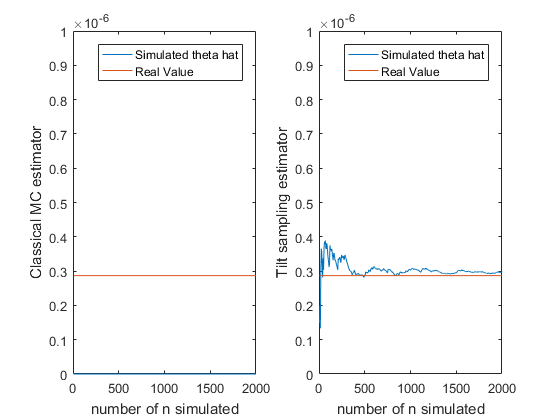
\includegraphics[scale=1]{hw1p1.png}

\bigskip
As you can see, classical MC failed even the n is 2000. This is because the probability of getting some random number bigger than 5 from standard normal distribution is very very unlikely. However, the tilted sampling works very fine and converge quickly after n is 500. So this proves the concept that the tilted sampling is better in estimating rare event.

All code please see 'https://github.com/rikku1983/STAT5376/blob/master/hw1.m'\\
\bigskip

Thanks!


\end{document}